\chapter{Analysis of Unencrypted Data Transmission on Open Networks}

In this section, we demonstrate the risks of transmitting sensitive information over unencrypted networks by simulating a scenario in which data is sent in plain text. This simulation aims to highlight the critical importance of encryption for securing communications in real-world applications.

\section{Setup and Methodology}

The experiment was conducted as follows:

\begin{enumerate}
    \item The encryption on the access point (AP) was disabled, rendering the network open and unprotected.
    \item Both an attacker device (the host computer) and a victim device were connected to this open network.
    \item On the attacker device, a simple HTTP website was hosted using Python with the following HTML code:
    
    \begin{adjustbox}{max width=\linewidth}
    \begin{lstlisting}[language=html]
    <!DOCTYPE html>
    <html lang="en">
    <head>
        <meta charset="UTF-8">
        <meta name="viewport" content="width=device-width, initial-scale=1.0">
        <title>HTTP Example</title>
    </head>
    <body>
        <h1>Welcome to an Unsecured HTTP Page</h1>
        <p>This is a demonstration of how data is sent in plain text over an unencrypted HTTP connection.</p>
        <form action="/submit" method="get">
            <label for="username">Username:</label>
            <input type="text" id="username" name="username">
            <br>
            <label for="password">Password:</label>
            <input type="password" id="password" name="password">
            <br>
            <button type="submit">Submit</button>
        </form>
    </body>
    </html>
    \end{lstlisting}
    \end{adjustbox}
    
    \item The victim device accessed the website through the open network and submitted credentials via the provided form.
    \item On the attacker device, Wireshark was used to capture and analyze the network traffic, revealing the transmitted username and password in plain text within an HTTP GET request.
\end{enumerate}

\section{Observed Results}

Using Wireshark, the attacker was able to intercept the network traffic and identify the HTTP GET request containing the user's credentials. Figure~\ref{fig:wireshark_capture} illustrates the intercepted request, showing the username and password in clear text. 

\begin{figure}[H]
    \centering
    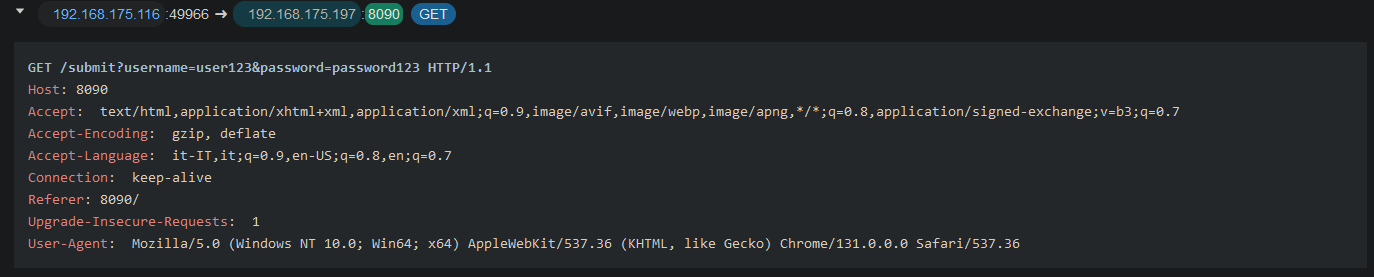
\includegraphics[width=\textwidth]{images/whiresharkcapture.png}
    \caption{Captured HTTP GET request showing transmitted credentials.}
    \label{fig:wireshark_capture}
\end{figure}

The lack of encryption allowed for the immediate identification of sensitive information, emphasizing the vulnerability of data transmission over open networks.

\subsection{Real-World Implications}

While this simulation was conducted in a controlled environment, it closely mimics real-world scenarios in which users connect to open networks, such as public Wi-Fi in cafes, airports, or other public spaces. In these environments, attackers can similarly exploit the absence of encryption to intercept sensitive information.

For example:
\begin{itemize}
    \item Users accessing websites without HTTPS encryption are vulnerable to attacks, such as credential theft or session hijacking.
    \item Even legitimate websites may inadvertently expose users if their login forms rely on HTTP instead of HTTPS.
\end{itemize}

This simulation underscores the vital importance of encryption protocols, such as HTTPS, in securing data transmission. By encrypting the content, these protocols ensure that sensitive information cannot be easily intercepted or interpreted, highlighting the indispensable role of cryptography in modern network security.


\section{Conclusion}

The experiment demonstrates how unencrypted networks pose significant risks to user data. It serves as a strong argument for adopting encryption protocols, such as WPA3 for wireless networks and HTTPS for web communication, to protect sensitive information.

Encryption is no longer optional but a fundamental requirement for ensuring data security in today's interconnected world.
